\documentclass[14pt]{extarticle}

\begin{document}
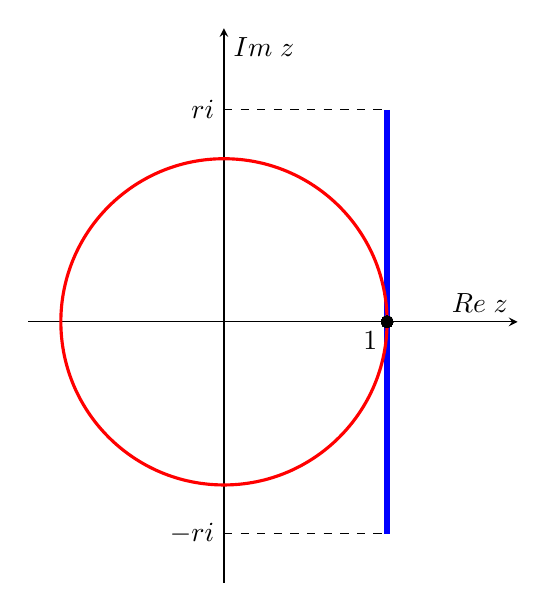
\begin{tikzpicture}
	\newcommand*{\Radius}{1.3}
	\begin{axis} [
		width  = 10cm,
		unit vector ratio*=1 1,
		xlabel = {$Re\;z$},
		ylabel = {$Im\;z$},
		xmin = -1.2,
		xmax = 1.8,
		ymin = -1.6,
		ymax = 1.8,
		axis x line = middle,
		axis y line = middle,
		ticks = none]

		\coordinate(A) at	(1, \Radius);
		\node[left](Ap) at	(0, \Radius) {$ri$};
		\coordinate(B) at	(1, -\Radius);
		\node[left](Bp) at	(0, -\Radius) {$-ri$};

		\draw[blue, line width=0.8mm]
			(A) -- (B);
		\draw[red, line width=0.4mm]
			(axis cs:0, 0) circle [radius=1];
		\draw[dashed] (Ap) -- (A) (Bp) -- (B);

		\node[below left] at	(1,0) {$1$};

		\addplot[mark=*,only marks, fill=black]
			(1, 0) node[above, pos=1]{};
	\end{axis}
\end{tikzpicture}
\end{document}
